\documentclass[main.tex]{subfiles} 
\begin{document}

\section*{Analyse}
\label{sec:2}

\subsection*{Aktivering av forkunnskaper (helklassesamtale)}
Ved oppstarten av timen initierte jeg dialog med elevene. Helklassesamtalene hadde preg av
IRE/F metoden (\citeNP{klet13}), dvs. lærer tar initiativ(I), elev responderer(R) og responsen blir 
evaluert(E) og/eller kommentert(F). Til denne sekvensen rakk elevene opp hånda for å respondere. 
Det viser seg at det er få elever som er villig til å svare, oftest de flinke elevene. Dette 
er uheldig siden flerparten av elevene ikke er aktive. Dermed får de ikke brukt denne sekvensen som
en anledning til å trene på å bruke naturfaglige begreper, som kunne kunne ha bidrat til å øke deres 
forståelse (\citeNP[s. 176]{klet13}).
\newline
\newline
Jeg brukte heller ikke ``revoicing'' tilstrekkelig gjennom denne sekvensen, til å gjenta og 
forsterke elevenes forslag. Ifølge Klette, viser fravær av slike eksplisitte 
innramminger fra lærerens side at eleven blir sittende med et uklart kunnskapsinnhold og i 
verste fall feil begrepsforståelse (\citeNP[s. 175-176]{klet13}). For å kunne bruke revoicing 
mest mulig effektivt, må læreren raskt kunne bestemme om elevens repons har validitet 
og om det er relevant. Gjennom egen prasiserfaring har revoicing vært vanskelig å utføre.
Ved å forutse elevsvar før elever i klassen blir initiert, kan misforståelser som ofte oppstår bli 
redegjort av læreren, og respons som ofte opptrer kan derfor tas stilling til. Dette krever imidlertid 
en god del erfaring fra læreren sin side. I \citeA[s. ~401]{batp08} klassifiseres dette som 
``knowledge of content and students, (KCS)''. Over tid vil en lærer danne omfattende KCS og
dette kan dermed bidra til å øke kvaliteten på helklassesamtalene. Revoicing kan også brukes
i andre sammenhenger, for eksempel i neste del av timen hvor jeg innførte et nytt tema. 

\subsection*{Innføring av nytt tema (forelesning)}
Ved innledning til temaet encellede organismer 
benyttet jeg anledningen til å aktivisere elevene ved å engasjere de i en dialog. For eksempel
når jeg snakket om bakterier, stilte jeg spørsmål som ``Kan dere fortelle meg om noen bakterier dere kjenner
til?'', ``Hvorfor vasker vi våre hender når vi har vært på do?'', og ``Er alle bakterier skadelig for mennesker?''.
Til det siste spørsmål var mange elever av oppfatning at bakterier er ``ting'' som skader mennesker og at vi
må aktivt søke beskyttelse fra disse organismene. Slike anledninger er fint å bruke til å rette opp 
misforståelser og tilføre nytt informasjon. For eksempel, til respons fortalte jeg elevene om at deres
fordøyelsessystem består av billioner (en størrelsesorden som jeg måtte redegjøre for i timen) av bakterier 
som hjelper kroppen til å bryte ned maten. På denne måten danner elevene nye assosiasjoner til bakterier,
assosiasjoner som tidligere var negative.
\newline
\newline
Fra figur \ref{fig:odeg10} kan vi se at i en vanlig naturfagstime brukes mye tid på å formidle 
nytt fagstoff, og det er lite konsolideringssituasjoner, deriblant gjennomgang av lekser. Gjennom
min egen praksiserfaring forsøkte jeg å unnvike en slik tendens. Hensikten med timen var å øke begrepsforståelse 
blant elever, og ikke fokusere på innføring av nye temaer. Dessuten brukte jeg en større porsjon 
av timen til å repetere begrepene elevene hadde hatt om celler og celledeling. I
tokolonnenotatet øvelsen skulle elevene få muligheten til å konsolidere alt de har lært hittil
om celler, inkludert innføringen av begrepet encellede organismer. Derfor ble tokolonnenotat 
øvelsen en naturlig avslutning til timen.


\begin{figure}[h!]
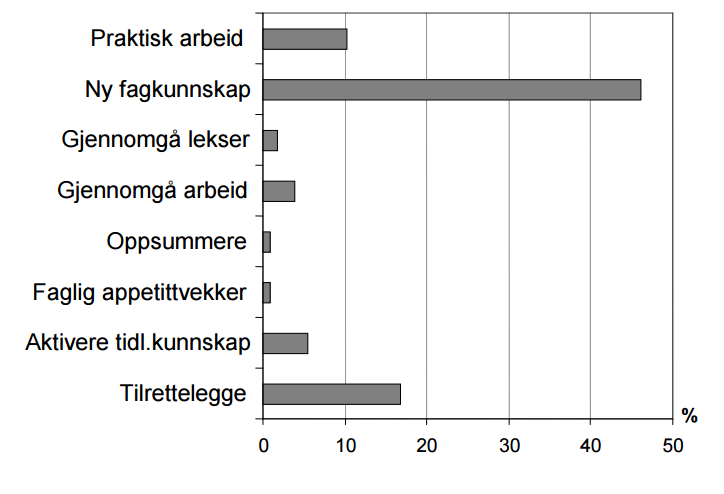
\includegraphics[scale = 0.6]{../figures/undervisnings_aktivitet.png}
\caption{Oversikt over naturfaglærernes undervisningstilbud til elevene fra PISA+ studie. Kilde: 
\protect\citeA{odeg10}.}
\label{fig:odeg10}
\end{figure}

\subsection*{Gruppesamtaler (samarbeid vs. kollaborasjon)}
Den sosiokulturelle teorien har utgangspunkt i Lev Vygotsky sine perspektiver på læring og 
utvikling (\citeNP[s. 13]{meli07}; \citeNP[s. 123]{bta98}; \citeNP[s. 87]{rogs13}; 
\citeNP[s. 299]{sjob04}; \citeNP[s. 62]{knai11}). Vygotskys 
mente at barns intellektuelle utvikling er formet utfra tilegnelse av språk, fordi språk 
muliggjør dialog mellom mennesker (\citeNP[s. 5]{meli07}). Dette har senere fått empirisk
støtte, og har derfor implikasjoner for utdanningsteori og -praksis (\citeNP[s. 83]{meli07}).
\newline
\newline
I helklassesamtalen ved starten av timen var det bare et fåtall elever som var aktive i lærerinitiert 
dialog. Dette var uheldig siden elevenes styrker og svakheter ikke ble tilstrekkelig avdekket. 
Gruppesamtalene viste seg å være en god plattform for å avdekke hull og svakheter i elevenes 
begrepsbruk. I den forbindelse ble tokolonnenotatet tatt i bruk (se vedlegg: \ref{sec:tokolonnenotat}).
\newline
\newline
I tokolonnenotatøvelsen viste noen grupper akkumulative tendenser. Det vil si at elevene 
var villige til å akseptere hverandres bidrag uten å stille kritiske spørsmål og fremsette
alternative eller utfyllende forklaringer. Noen elever som jobbet i en gruppe, arbeidet så og si
selvstendig ved å føre rett inn i sine egne utdelte kopier av tokolonnenotatet. Et sluttresult som 
ikke var basert på et felles grunnlag. Dermed fikk de en annen type utbytte fra gruppearbeidet
enn det som var tiltenkt, hva \citeNP[s. 25]{meli07}  definerer som ``groupsense or feeling of a shared endeavour''. 
Med andre ord ble det et samarbeid og ikke en kollaborasjon, som \citeA{meli07} respektivt kaller 
\emph{interacting vs. interthinking}. Gruppen endte opp med et felles produkt, men det var ikke 
basert på en kollaborasjon mellom elevene. Målet med et samarbeid er å ende opp med et sluttprodukt. 
I motsetning er en kollaborasjon der individer frembringer egene ideer til gruppen, og hver ide
blir da vurdert og diskutert felles i gruppen: enten blir den akseptert eller så forkastes den.
\newline
\newline
En viktig del av den sosiale utprøvingen av ideer og begreper innebærer å sammenlikne egne 
forestillinger med andres forestillinger i tillegg til naturvitenskapens forklaringer 
(\citeNP{odeg10}; \citeNP{dals94}). Bruken av tokolonnenotatet i første timen 
\newline
\newline
Når elevene ble deretter fordelt i andre grupper og prøvde å presentere begrepene, viste noen elever 
svak forståelse. I blant ble begrepene fremstilt overfladisk, og for noen elever ble deres svakheter 
om temaene avdekket. Noen elever misbrukte øvelsen til en viss grad ved å avskrive notatene til sine 
medelever. Til deres forsvar kan det sies at instruksene som ble formidlet ikke var tydelige nok. 
Uansett ble denne oppførselen irettesatt og klarere instrukser ble formidlet.
\newline
\newline
Min rolle som lærer til denne øvelsen lå i veilede elevene i den nærmeste utviklingssonen.
Den \emph{nærmeste utviklingssonen} beskriver en sone som ligger i mellom et barns kognitive 
ferdigheter, dvs. hva de kan oppnå selvstendig uten hjelp, og dets potensielle utvikling, dvs. 
hva en elev kan få til eller forstå gjennom enten veiledning eller kollaborasjon 
(\citeNP[s. 14]{meli07}; \citeNP[s. 125]{bta98}; \citeNP[s. 75]{rogs13}). Jeg brukte ``scaffolding'' 
eller stillasbygging (\citeNP{bta98}; \citeNP[s. 71]{math15}) for å knytte begrepene til elevenes 
forkunnskaper og hverdagsoppfatninger. Gode fagsentrerte samtaler mellom elever (eller faglige samtaler 
med lærer) hvor elever bruker egne erfaringer og språket for å oppnå faglig forståelse hjelper til å 
skape bro mellom praksis og teori (\citeNP{odeg10}).
\newline
\newline
I kognitiv konstruktivisme utgjør elevenes erfaringer og kunnskaper det de kan møte nye 
utfordringer med. Piaget kaller delstrukturer som utgjør disse kognitive strukturene 
for (mentale) skjemaer (\citeNP[s. 78]{solv92}). Piaget mente at elevenes tenkning ble 
utviklet gjennom to forskjellige typer prosesser: ``assimilasjon'' og ``akkomodasjon'' 
(\citeNP[s. 65]{rogs13}). I den første prosessen utvider elevene sine skjemaer, men
det skjer ingen endring. Når elevene møter noe som ikke stemmer overens med de
eksisterende skjemaer, endres skjemaene, altså akkomodasjon. Det er gjennom en 
kombinasjon av begge prosessene at elevene anskaffer den ønskelige type kunnskap,
operativ kunnskap, i motsetning til figurativ kunnskap.
\newline
\newline
Evnen til abstrahering henger ifølge Vygotsky (\citeNP[s. 127]{bta98}) sammen med begrepsundervisning, som en
form for vitenskapeliggjøring av hverdagsbegreper. Hvis elever ikke har god begrepsforståelse
kan de ende opp med å bruke naturvitenskapelige begreper i feil kontekst og danne feil 
forbindelser med begrepene. Dette avhenger av deres forkunnskaper. Ausubels kognitive bruer 
(\citeNP[s. 71]{math15}), hans teori om begrepslæring på høyere nivå og hvordan læreren best kan 
legge til rette for slik læring og bruk av begrepene, handler om å danne forbindelser mellom 
undervisningsmateriell og relevante ideer i elevenes kognitive struktur.

\end{document}